\documentclass{beamer}

\title{Memory Management in the Cloud}
\author{Saurabh Mathur\\ 
\emph{saurabhmathur96@gmail.com}}

\institute{ SITE, VIT Vellore }
\date{\today}

\usetheme{Madrid}
\usecolortheme{whale}

\begin{document}

\begin{frame}
\maketitle
\end{frame}

\begin{frame}
\frametitle{Definition}
\begin{block}{Cloud Computing}
A kind of Internet-based computing that provides shared processing resources and data to computers and other devices on demand.
\end{block}
\end{frame}


\begin{frame}

\frametitle{The Cloud Computing Stack}
\begin{center}
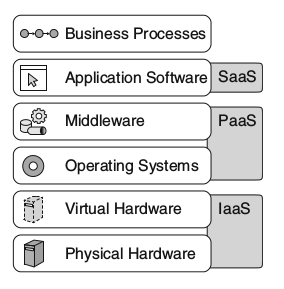
\includegraphics[width=.5\textwidth]{stack}
\end{center}

\end{frame}

\begin{frame}

\frametitle{The Cloud Computing Stack}
\begin{center}
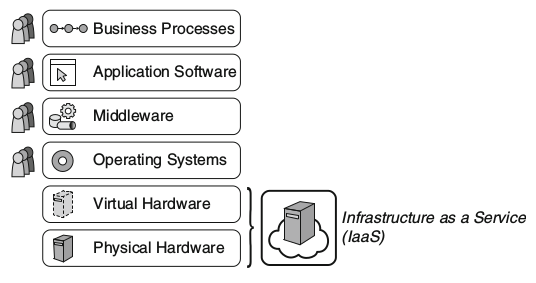
\includegraphics[width=\textwidth]{IaaS}
\end{center}

\end{frame}

\begin{frame}

\frametitle{The Cloud Computing Stack}
\begin{center}
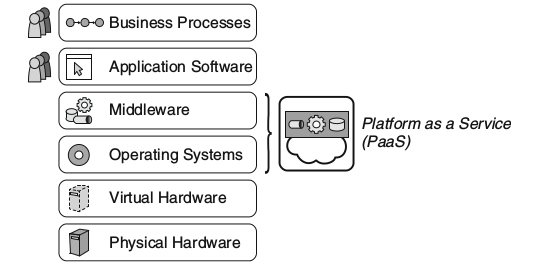
\includegraphics[width=\textwidth]{PaaS}
\end{center}

\end{frame}

\begin{frame}

\frametitle{The Cloud Computing Stack}
\begin{center}
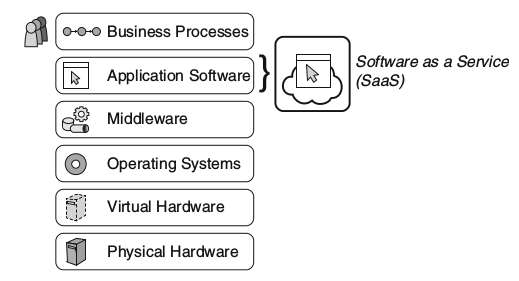
\includegraphics[width=\textwidth]{SaaS}
\end{center}

\end{frame}

\begin{frame}
\frametitle{Characteristics}
\begin{itemize}
\item Reduction in capital expenditure
\item Device and location independence
\item Sharing of resources (and costs)
\item Centralization of infrastructure and data
\item Reliability by way of multiple redundant sites
\item Scalability

\end{itemize}

\end{frame}

\begin{frame}

\frametitle{Memory Management}
\begin{center}
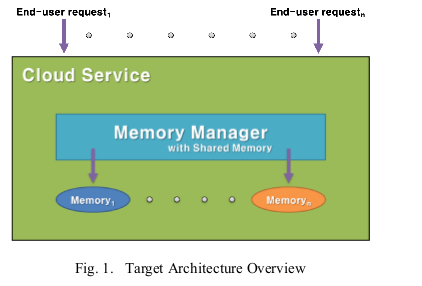
\includegraphics[width=\textwidth]{memory-arch}
\end{center}

\end{frame}


\begin{frame}

\frametitle{Page Replacement}
\begin{center}
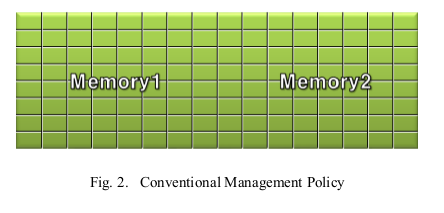
\includegraphics[width=\textwidth]{conventional}
\end{center}

\end{frame}


\begin{frame}

\frametitle{Static Partitioning}
\begin{center}
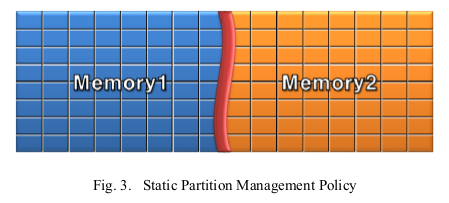
\includegraphics[width=\textwidth]{static}
\end{center}

\end{frame}

\begin{frame}
\frametitle{Static Partitioning}
\begin{itemize}
\item Every memory is divided statically by predefined partition ratio
\item Simple implementation
\item Less Overhead
\item Calculation needs to be done beforehand
\item Memory is wasted


\end{itemize}

\end{frame}


\begin{frame}

\frametitle{Dynamic Partitioning}
\begin{center}
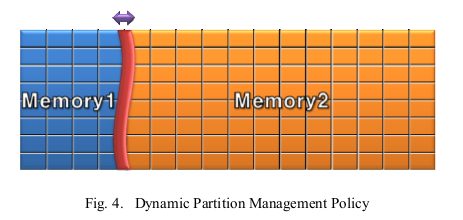
\includegraphics[width=\textwidth]{dynamic}
\end{center}

\end{frame}




\begin{frame}
\frametitle{Dynamic Partitioning}
\begin{itemize}
\item Every line of shared memory is divided dynamically depending on the number of misses for each memory
\item Efficient in terms of memory
\item Overhead due to calculation
\item No calculation required before deployment
\item 4.65\% performance boost 
 

\end{itemize}

\end{frame}


\begin{frame}
\frametitle{Static Partitioning - Statistics}
\begin{center}
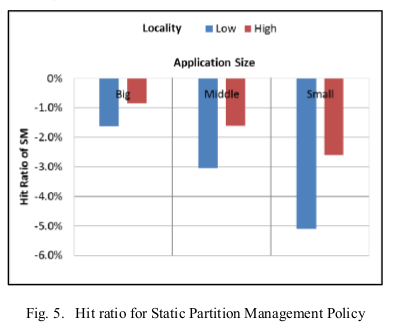
\includegraphics[width=.6\textwidth]{static-stat}
\end{center}

\end{frame}



\begin{frame}

\frametitle{Dynamic Partitioning - Statistics}
\begin{center}
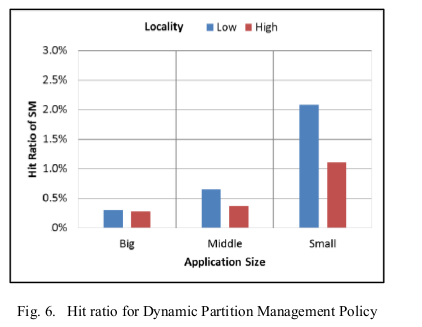
\includegraphics[width=.6\textwidth]{dynamic-stat}
\end{center}

\end{frame}

\begin{frame}

\frametitle{References}
\begin{itemize}
\item \textit{Analysis of Memory Management Policies for Heterogeneous Cloud Computing}, Dong Oh Son et al.
\item  \textit{Cloud Computing Patterns}, C. Fehling et al.

 

\end{itemize}

\end{frame}






\end{document}